\documentclass[11pt]{article}
\usepackage[margin=1in]{geometry}
\usepackage{amsmath,amssymb}
\usepackage{booktabs}
\usepackage{graphicx}
\usepackage{xcolor}
\usepackage{caption}
\usepackage[most]{tcolorbox}
\usepackage{enumitem}
\usepackage{hyperref}
\hypersetup{colorlinks=true,linkcolor=blue,citecolor=blue}

\newtcolorbox{figbox}[1]{colback=gray!6,colframe=gray!50,title={#1},
  fonttitle=\bfseries\small,boxrule=0.5pt,arc=2pt,left=4pt,right=4pt,top=3pt,bottom=3pt}

\title{\vspace{-2em}Multi-Agent Item Generation and Expert-Free Critic Validation\\
\large (Methods \& Results excerpt for the NCT paper --- drop-in for the \textsc{.docx})}
\author{}
\date{}

\begin{document}
\maketitle
\vspace{-3em}

\noindent\textbf{How to use this file.} Everything below maps 1:1 to the
\emph{Materials and Methods} and \emph{Result and Discussion} sections.
Grey boxes mark where to paste a figure/screenshot. All numbers and tables are
the real results from our runs.

% =====================================================================
\section{Materials and Methods}

\subsection{System overview}
We frame item generation as a two-agent loop. A \emph{Generator} agent
$G$ proposes a multiple-choice item; a \emph{Critic} agent $C$ scores it on
several pedagogical dimensions and either accepts it or returns targeted
feedback, in which case $G$ regenerates (up to $R$ retries). For mathematics, a
deterministic \emph{symbolic verifier} runs before the critic. The accepted
item, its critic verdict, and (in ensemble mode) the per-critic breakdown are
persisted as JSON and Markdown.

\begin{figbox}{Fig.~1 --- INSERT: agent workflow diagram}
A block diagram: \textsf{Generator $G$} $\rightarrow$ (math only)
\textsf{Symbolic verifier} $\rightarrow$ \textsf{Critic / 3-model ensemble}
$\rightarrow$ decision $\langle$\textsf{pass}$\rangle$ store, or
$\langle$\textsf{fail}$\rangle$ feedback loop back to $G$. Annotate the loop with
``$\le R$ retries''. \emph{Recommended: draw in draw.io / PowerPoint, export PNG.}
\end{figbox}

\subsection{Models and infrastructure}
All agents are LLMs served through OpenRouter. We evaluate three frontier
models as both generators and critics: \textsc{Gemini-3.1-Pro},
\textsc{GPT-5.5}, and \textsc{Claude-Sonnet-4.6}. The generator samples at
temperature $0.8$ (diversity); the critic samples at $0.2$ (stable scoring).
Outputs are constrained to JSON.

\subsection{Item specification and alignment to the national test}
We align generation to the official National Testing Center (NTC,
\emph{Ulttyq testileu ortalygy}) teacher-certification specification. Each test form has
$50$ items: $40$ standalone items and $10$ context-based items organised as two
shared-passage blocks of five questions each. Difficulty follows the official
mix---basic (A), medium (B), hard (C)---in the proportions
\[
p_A = 26\%,\qquad p_B = 60\%,\qquad p_C = 14\%.
\]
For a batch of $N$ items the per-level counts use largest-remainder rounding,
\(
n_\ell = \operatorname{round}(p_\ell N),\ \sum_\ell n_\ell = N .
\)
Topics follow the specification: $10$ Kazakh-language topics (phonetics and
orthography $\rightarrow$ lexicology $\rightarrow$ morphology $\rightarrow$
syntax $\rightarrow$ style/text analysis) and $20$ mathematics topics.

\subsection{Generator agent}
The generator prompt is templated by subject, topic, and difficulty, and
injects $k$ few-shot exemplars retrieved from \emph{real} published items of
the same subject (and, for context blocks, anchored on a real context block).
The model returns the stem, four options, the key, and an explanation.

\begin{figbox}{Listing 1 / Fig.~2 --- INSERT: example prompt + generated item}
Paste one generator prompt (system message) and one resulting JSON item
(e.g., a Kazakh lexicology item or a context block of five questions).
\emph{Use a monospaced screenshot or a shaded verbatim box in the \textsc{.docx}.}
\end{figbox}

\subsection{Critic agent and the multi-critic ensemble}
The critic first solves the item independently, then scores it on five
dimensions $d\in\mathcal D=\{$correctness, distractor quality, difficulty
alignment, language quality, \LaTeX/figure validity$\}$, each in $[0,10]$. The
overall score is a weighted mean
\begin{equation}
S \;=\; \frac{\sum_{d\in\mathcal D} w_d\, s_d}{\sum_{d\in\mathcal D} w_d},
\qquad (w_{\text{correctness}}=3,\ w_{\text{others}}\in\{1,2\}),
\label{eq:score}
\end{equation}
and the item passes when $S \ge \theta$ (we use $\theta = 6.0$).

\paragraph{Ensemble (contribution 1).} To reduce single-model
self-evaluation bias we aggregate $K=3$ critics. For the answer we take the
majority vote $a^\star=\operatorname{mode}\{a^{(1)},\dots,a^{(K)}\}$ with
agreement $\alpha=\frac1K\sum_k \mathbf 1[a^{(k)}=a^\star]$; each dimension is
the mean $\bar s_d=\frac1K\sum_k s_d^{(k)}$. Pairwise inter-critic reliability
is reported with Cohen's $\kappa$,
\begin{equation}
\kappa \;=\; \frac{p_o - p_e}{1 - p_e},
\label{eq:kappa}
\end{equation}
where $p_o$ is observed and $p_e$ chance agreement on the chosen option.

\subsection{Symbolic verification for mathematics (contribution 2)}
For mathematics the generator may emit a machine-checkable specification that
is evaluated in a sandboxed \textsc{SymPy} process \emph{before} the LLM critic.
The verifier recomputes the answer symbolically; its verdict
$v\in\{$confirmed, contradicted, inapplicable$\}$ is injected into the critic
prompt as authoritative evidence, making correctness judgements
model-independent for the items it covers.

\subsection{Vision-aware critic}
Figure-dependent (image) mathematics items are routed to a vision-capable
critic that receives the rendered figure as a multimodal input; text items use
the cheaper text critic. This ensures the critic can actually \emph{see} the
figure it is grading.

\subsection{Expert-free critic validation: the Critic Discrimination Index (contribution 3)}
We validate a critic \emph{without} human grading by injecting known quality
faults and measuring whether the critic detects them. From each real item we
synthesise two degraded variants: \textsc{wrong-key} (the key is relabelled to
a distractor) and \textsc{weak-distractors} (two distractors are replaced by
implausible fillers). For dimension $d$ the \emph{Critic Discrimination Index}
is the paired mean drop
\begin{equation}
\mathrm{CDI}_d \;=\; \frac{1}{N}\sum_{i=1}^{N} s_d^{\text{real}}(i)
\;-\; \frac{1}{N}\sum_{i=1}^{N} s_d^{\text{deg}}(i).
\label{eq:cdi}
\end{equation}
A well-calibrated critic yields a \emph{large positive} $\mathrm{CDI}_d$ on the
dimension the degradation targets (e.g.\ wrong-key $\rightarrow$ correctness)
and $\mathrm{CDI}_d\!\approx\!0$ elsewhere (discriminant validity). Significance
is assessed with the two-sided Wilcoxon signed-rank test, and effect size with
the paired Cohen's $d$,
\begin{equation}
d \;=\; \frac{\overline{\Delta}}{s_\Delta},\qquad
\Delta_i = s_d^{\text{real}}(i) - s_d^{\text{deg}}(i),
\label{eq:cohend}
\end{equation}
where $\overline{\Delta}$ and $s_\Delta$ are the mean and standard deviation of
the paired differences ($d>0.8$ is conventionally a large effect).

% =====================================================================
\section{Result and Discussion}

\subsection{The critics discriminate quality (CDI)}
Tables~\ref{tab:cdi-math} and~\ref{tab:cdi-kz} report CDI for the targeted
dimensions across the three critics. On both subjects and for all three models
the discrimination is \emph{statistically significant} with \emph{large} effect
sizes: relabelling the key collapses the correctness score, and weakening the
distractors collapses the distractor-quality score, exactly as a valid critic
should behave. Figure~\ref{fig:cdi} visualises the gaps.

\begin{table}[h]
\centering
\caption{CDI on \textbf{mathematics} ($N\!\approx\!40$ real items per model;
all $p<0.001$, Wilcoxon).}
\label{tab:cdi-math}
\begin{tabular}{lccc}
\toprule
Critic & Solve acc. & wrong-key $\rightarrow$ correctness & weak-distr. $\rightarrow$ distractor q. \\
       &            & gap ($d$) & gap ($d$) \\
\midrule
Claude-Sonnet-4.6 & 0.98 & $+8.85\ (4.94)$ & $+3.03\ (1.53)$ \\
Gemini-3.1-Pro    & 0.95 & $+8.58\ (2.95)$ & $+5.10\ (1.50)$ \\
GPT-5.5           & 1.00 & $+8.73\ (2.75)$ & $+2.99\ (1.69)$ \\
\bottomrule
\end{tabular}
\end{table}

\begin{table}[h]
\centering
\caption{CDI on \textbf{Kazakh language} ($N\!=\!20$ real items per model;
all $p\le 0.0002$, Wilcoxon).}
\label{tab:cdi-kz}
\begin{tabular}{lccc}
\toprule
Critic & Solve acc. & wrong-key $\rightarrow$ correctness & weak-distr. $\rightarrow$ distractor q. \\
       &            & gap ($d$) & gap ($d$) \\
\midrule
Claude-Sonnet-4.6 & 0.75 & $+5.15\ (1.73)$ & $+4.60\ (3.87)$ \\
Gemini-3.1-Pro    & 0.90 & $+8.15\ (1.87)$ & $+7.90\ (4.07)$ \\
GPT-5.5           & 0.80 & $+6.70\ (1.69)$ & $+3.90\ (2.99)$ \\
\bottomrule
\end{tabular}
\end{table}

\begin{figure}[h]
\centering
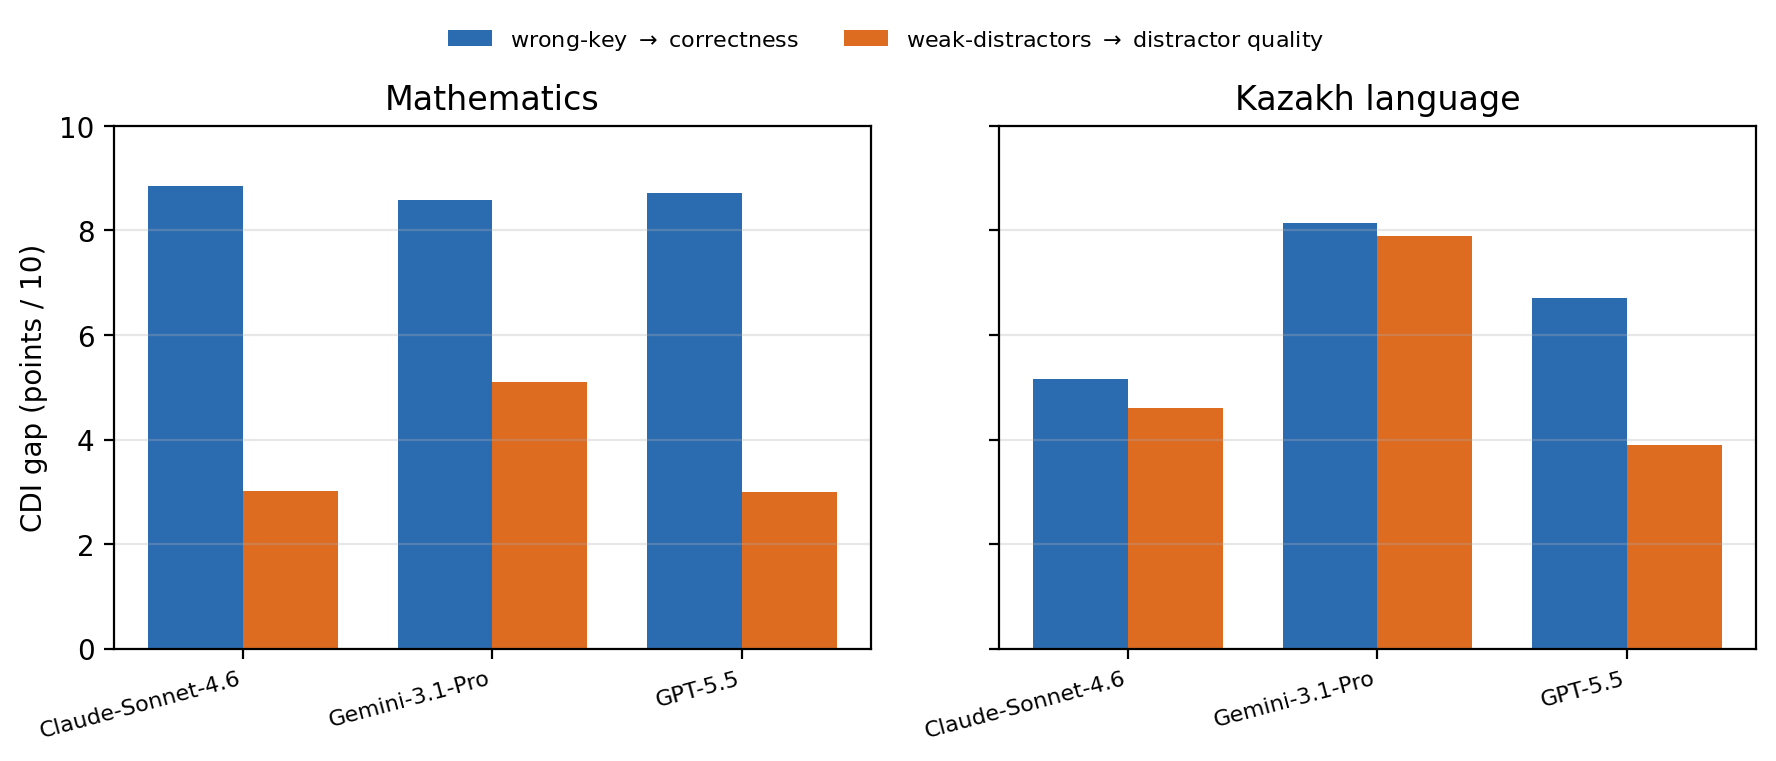
\includegraphics[width=\linewidth]{fig_cdi.png}
\caption{Critic Discrimination Index (gap between real and degraded mean
scores) for the targeted dimensions, by model and subject. Larger is better;
all gaps are statistically significant.}
\label{fig:cdi}
\end{figure}

\subsection{Inter-critic agreement}
On real items the three critics agree on the answer with high frequency; we
report pairwise Cohen's $\kappa$ (Eq.~\ref{eq:kappa}) computed on the
ensemble's chosen options.
\begin{figbox}{INSERT: Cohen's $\kappa$ values}
Fill from the ensemble run's \texttt{pairwise\_kappa}
(\texttt{summary.json}). One small table: critic-pair $\times$ $\kappa$.
\end{figbox}

\subsection{Vision matters for figure items (ablation)}
On the figure-dependent mathematics items, critics evaluated \emph{without} the
image (text only) answered $6/9$ correctly across the three models, whereas with
the figure supplied to the vision critic they answered $9/9$
(Table~\ref{tab:vision}). This isolates the value of the vision-aware routing.
The sample is small ($n=3$ image items per model) and is reported as a
controlled sanity check rather than a powered comparison.

\begin{table}[h]
\centering
\caption{Vision ablation on figure-dependent mathematics items.}
\label{tab:vision}
\begin{tabular}{lcc}
\toprule
Critic & Blind (no image) & With image \\
\midrule
Claude-Sonnet-4.6 & $2/3$ & $3/3$ \\
Gemini-3.1-Pro    & $1/3$ & $3/3$ \\
GPT-5.5           & $3/3$ & $3/3$ \\
\midrule
\textbf{Total}    & $\mathbf{6/9}$ & $\mathbf{9/9}$ \\
\bottomrule
\end{tabular}
\end{table}

\subsection{Generated item bank}
Using the validated ensemble critic we generated a full Kazakh-language bank of
$150$ items (three models $\times\,50$), Table~\ref{tab:bank}. Standalone items
passed the ensemble at $120/120$ with a mean overall score of $9.14/10$; for the
six context blocks the ensemble's independent answer matched the generated key
on all $30/30$ questions.

\begin{table}[h]
\centering
\caption{Generated Kazakh item bank (3 models $\times$ 50; ensemble critic).}
\label{tab:bank}
\begin{tabular}{lccc}
\toprule
Type & Items & Critic--key match & Passed \\
\midrule
No-context (standalone) & $120$ & --- & $120/120$ \\
With-context (6 blocks) & $30$  & $30/30$ & $30/30$ \\
\midrule
\textbf{Total} & $\mathbf{150}$ & & \\
\bottomrule
\end{tabular}
\end{table}

\begin{figbox}{INSERT (optional): example generated context block}
Paste one passage + its five questions (Kazakh) as an illustrative example,
with the ensemble score and agreement per question.
\end{figbox}

\subsection{Discussion and limitations}
The results support three claims: (i) a multi-agent generate--critique pipeline
produces national-test-aligned items in a low-resource language at high accepted
quality; (ii) CDI validates the critic \emph{without} expert grading, showing
significant, large-effect discrimination on both subjects; and (iii) an ensemble
of heterogeneous critics plus symbolic verification reduces single-model bias.
Limitations to state honestly: CDI is a \emph{proxy} for human judgement
(expert-correlation is future work); the vision ablation ($n=3$) and the single
real context block limit statistical power for those specific analyses; and the
generated bank is validated by the automated critic rather than by human
experts, which we plan to address with a targeted expert review.

\end{document}
